\documentclass{beamer}[UTF-8]
\usepackage{ctex}
\usepackage{graphicx}
\usepackage{listings}
\usepackage{fontspec}
\setmonofont{Fira Code}
\usetheme{CambridgeUS}
\setCJKsansfont{SimSun}


\title{Lesson 1——基础算法复习}
\subtitle{NOIP非基础新课}
\author{Garen Wang}
\date{\today}

\begin{document}
% 标题页
\maketitle

\begin{frame}{目录}
需要讲的知识点一共有下面这些: \pause
\tableofcontents
\end{frame}

\section{模拟} % 模拟
\begin{frame}{模拟}
\begin{center} 以那暴力模拟向正解吊唁 ——《膜你抄》 \end{center}

\begin{itemize}
\item 模拟就是题目叫你做什么你就做什么。  \pause
\item 一般的道理就是把整个算法过程都说给你听,然后请你实现。   \pause
\item 模拟题在实现方面一般没有多大难度,但是需要对题意有充分的了解。  \pause
\item 总之一句话:注意细节!  \pause
\item 细节做的不好的话可能让你去掉一大半分数。
\end{itemize}

\end{frame}

\begin{frame}{例题1:luoguP1015}
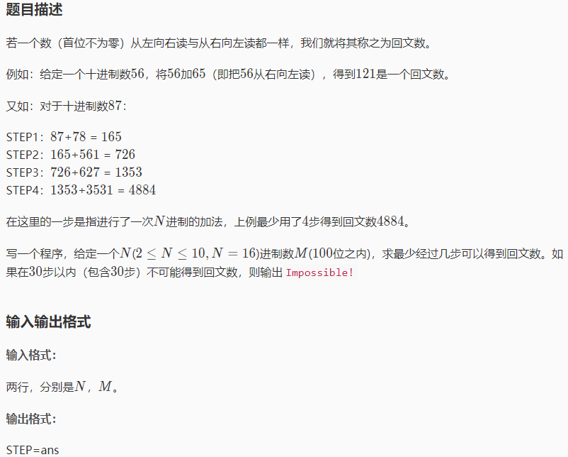
\includegraphics[width=\textwidth, height=\textheight]{luoguP1015.png}
\end{frame}

\begin{frame}{例题1——分析}
\pause
\begin{itemize}
\item 无f**k说。直接模拟就好了。  \pause
\item 求一个数的回文数都懂吧。。。
\end{itemize}
\end{frame}

\begin{frame}{例题2:某题}
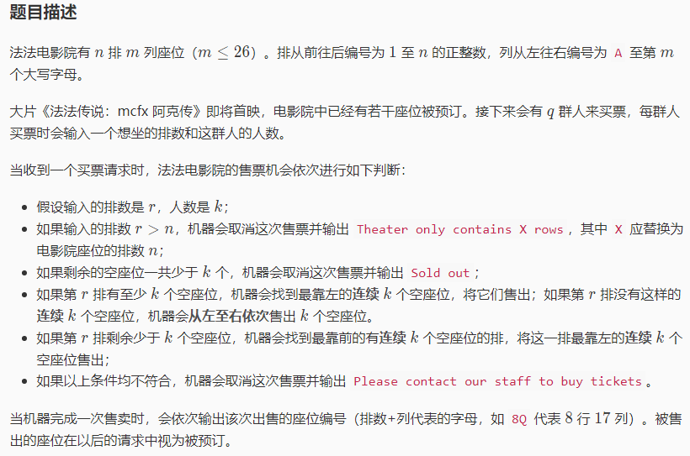
\includegraphics[width=\textwidth, height=\textheight]{temp1.png}
\end{frame}

\begin{frame}{例题2:某题}
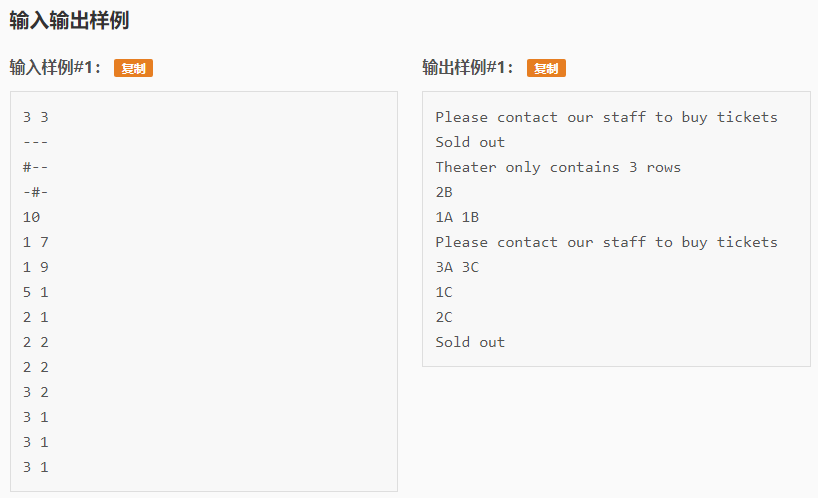
\includegraphics[width=\textwidth, height=\textheight]{temp2.png}
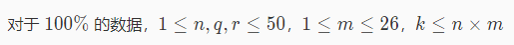
\includegraphics[width=\textwidth, height=\textheight]{temp3.png}
\end{frame}
\begin{frame}{例题2——分析}
 \pause
\begin{itemize}
\item 这道题就是真实的模拟。 \pause
\item 照着题意做,认真读题后再做。 \pause
\item 最后,注意数据范围,开好数组。 \pause
\item 然后就没事了。 \pause
\item 因为这道题不是公开题,所以想提交的qq发给我,我帮你交上去。
\item 我就不提供代码了。注意一下就能写。
\end{itemize}
\end{frame}

\begin{frame}{作业}
 \pause
\begin{itemize}
\item luoguP1003 铺地毯
\item luoguP1009 阶乘之和
\item luoguP1014 Cantor表
\item luoguP1076 寻宝
\item luoguP1328 生活大爆炸版剪刀石头布
\end{itemize}

\end{frame}

\section{暴力} % 暴力
\begin{frame}{暴力}
\begin{center} 骗分过样例,暴力出奇迹 \end{center} \pause
\begin{itemize}
\item 外国真的有这门算法,名字叫brute force。 \pause
\item 能用暴力做的题的前提是数据范围极其极其小。 \pause
\item 一般暴力可以用来找规律。有些结论题可以用暴力猜规律。 \pause
\item 优秀的码暴力能力是学习其他算法的坚实基础。
\end{itemize}
\end{frame}

\begin{frame}{例题1:luoguP1024}
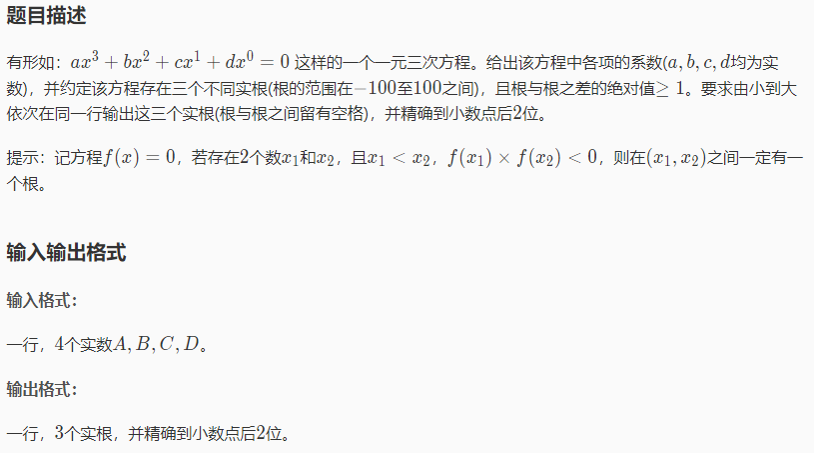
\includegraphics[width=\textwidth, height=\textheight]{luoguP1024.png}
\end{frame}

\begin{frame}{例题1——分析}
 \pause
\begin{itemize}
\item 这道题为什么可以暴力而不TLE呢?原因就在于: \pause
\begin{enumerate}
\item 根的范围在$-100$至$100$之间 \pause
\item 精确到小数点后两位 \pause
\end{enumerate}
\item 这意味着我们只需要判断$10000$个$x$是否合法即可。 \pause
\item 所以解决的方法就是找到三个$f(x)=0$的$x$即可。 \pause
\item 唯一要注意的就是浮点数的精度问题,判断零点还不能看是否等于$0$。 \pause
\item 代码不贴。
\end{itemize}
\end{frame}

\begin{frame}{例题2:luoguP1149}
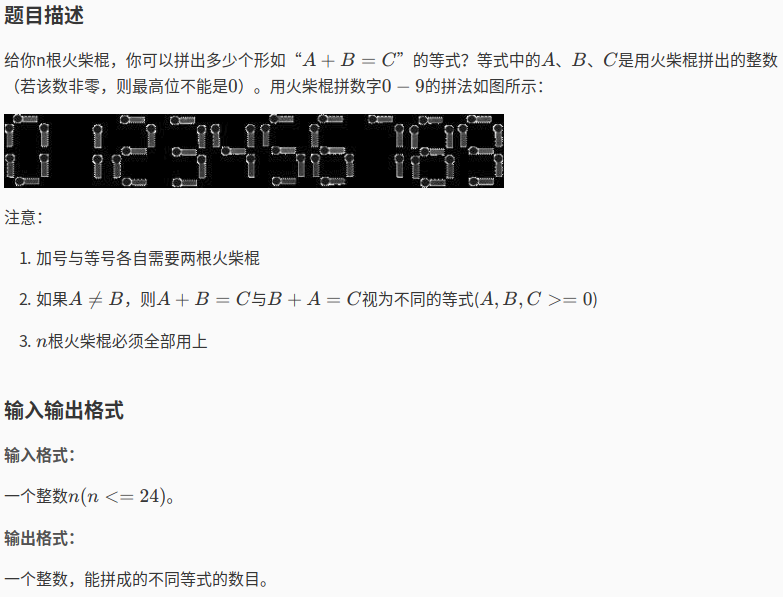
\includegraphics[width=\textwidth, height=\textheight]{luoguP1149.png}
\end{frame}

\begin{frame}{例题2——分析}
 \pause
\begin{itemize}
\item 思路比较简单:枚举两个加数,那么和就唯一确定,判断能否成立即可。 \pause
\item 这道题的难点就是你不知道枚举到多少才能枚举完。 \pause
\item (参照题解)发现可以把所有符合的等式都打出来,看看我们有必要枚举到哪个地方。  \pause
\item 听说答案是$711$。当然大于$711$不TLE的程序都是能过的。 \pause
\item 判断过程可以写个函数方便操作。 \pause
\item 代码一大堆,不贴。
\end{itemize}
\end{frame}

\begin{frame}{作业}
 \pause
找不到什么作业啊!!!所以就把一些显然的题目给大家。 \pause
\begin{itemize}
\item luoguP1097 统计数字 \pause
\item luoguP1088 火星人 \pause
\item CF1100A Roman and Browser \pause
\end{itemize}
\end{frame}
\section{二分} % 二分
\begin{frame}{二分}
 \pause
\begin{itemize}
\item Binary search是比较简单的带$\log$的算法,所以比暴力要快得多。数据越大越明显。 \pause
\item 生活例子:猜数字炸弹、翻字典 \pause
\item 二分的流程是这样的:(对区间$[l,r]$进行操作) \pause
\begin{enumerate}
\item 计算$l$和$r$的中点为$mid$。 \pause
\item 判断$mid$是否满足条件,如果符合,将区间往不符合方向移动;否则,向符合方向移动。移动方式是修改端点值。 \pause
\item 一直做2过程直到$l$和$r$不表示区间(可理解为$l>r$)为止。
\end{enumerate}
\end{itemize}
\end{frame}

\begin{frame}{二分的前提}
 \pause
\begin{itemize}
\item 使用二分是有前提的:条件的符合情况一定要具有单调性。 \pause
\item 在数组里找到小于等于$val$的最后一个元素,即std::lower\_bound操作。前提是要把数组排序。 \pause
\item 如果有一个问题,$val$越小越难满足,$val$越大越容易满足,那么jiushuo这个问题有单调性,可以二分。反之亦然。 \pause
\item 那我们二分能找到什么呢? \pause
\item 找到这个所谓的临界点。即“最小的最大”“最大的最小”。
\end{itemize}
\end{frame}

\begin{frame}{例题1}
 \pause
\begin{itemize}
\item 在数组里找到小于等于$val$的最后一个元素。 \pause
\item 首先先排序,满足大小的单调性,然后就可以二分了。 \pause
\item 这里给大家提供两个二分的模板,自行选用。 \pause
\item 镜像问题:在数组里找到大于$val$的第一个元素,即std::upper\_bound操作。
\end{itemize}
\end{frame}

\begin{frame}[fragile]{模板1}
    \pause
   模板1适用于浮点数。$left$和$right$就是前面所说的左右端点。 \pause
   \begin{lstlisting}[language = C++,
   numberstyle=\tiny,keywordstyle=\color{blue!70},
   commentstyle=\color{red!50!green!50!blue!50},frame=shadowbox,
   rulesepcolor=\color{red!20!green!20!blue!20},basicstyle=\ttfamily]
   ll left = 1, right = n;
   while(left < right) {
       ll mid = (left + right) / 2;
       if(a[mid] <= val) left = mid;
       else right = mid - 1;
   }
   \end{lstlisting}
   \end{frame}
   
   \begin{frame}[fragile]{模板2}
    \pause
   模板2只适用于整数类型。浮点数显然用不了这个,如果要用要写eps。 \pause
   \begin{lstlisting}[language = C++,
   numberstyle=\tiny,keywordstyle=\color{blue!70},
   commentstyle=\color{red!50!green!50!blue!50},frame=shadowbox,
   rulesepcolor=\color{red!20!green!20!blue!20},basicstyle=\ttfamily]
   ll left = 1, right = n, ans = -1;
   while(left <= right) {
       ll mid = (left + right) / 2;
       if(check(mid)) ans = mid, left = mid + 1;// 看单调性
       else right = mid - 1;// 同上
   }
   \end{lstlisting}
   \end{frame}

\begin{frame}{例题2:luoguP2678}
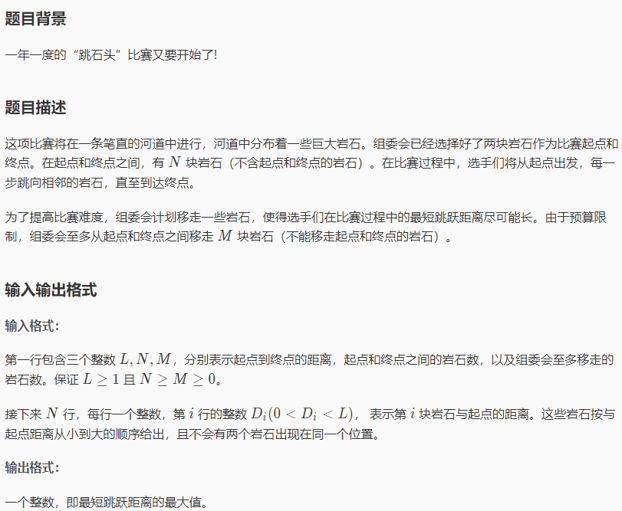
\includegraphics[width=\textwidth, height=\textheight]{luoguP2678.png}
\end{frame}

\begin{frame}{例题2——分析}
 \pause
\begin{itemize}
\item 这是二分在题目中的应用,叫做“二分答案”。顾名思义,就是通过发现答案具有单调性,从而对答案来二分。 \pause
\item 一眼看出题目考点:使得在比赛过程中的最短跳跃距离尽可能长。 \pause
\item 答案单调性:最短跳跃距离越短难度越小,越长则难度越大。 \pause
\item 所以套上二分的模板,具体化端点移动模式,然后就发现一个最大的问题: \pause
\item 你说的check函数怎么写啊?
\end{itemize}
\end{frame}

\begin{frame}{例题2——分析}
 \pause
\begin{itemize}
\item 二分答案的本质是把临界问题转变为判定问题。 \pause
\item check函数应为:当最短跳跃距离为$mid$时,选手能否完成比赛。 \pause
\item 显然check函数返回bool,能完成返回true,不能就返回false。 \pause
\item 假设现在拿到最短跳跃距离,该如何安排石头? \pause
\item 显然,要判断与前边已放石头的距离是否大于等于答案。如果可以,石头可以保留;否则,这块要拿走,看下一个石头能否放置。 \pause
\item 其实这里用到贪心的思想,我们建立满足答案的拿走最少的局面。 \pause
\item 以上就是check函数的写法。check函数的写法常常是一种贪心。
\end{itemize}
\end{frame}

\begin{frame}{作业}
 \pause
\begin{itemize}
\item luoguP1316 丢瓶盖
\item luoguP1024 一元三次方程求解(提示:极点之间的区域来二分)
\item luoguP1083 借教室
\item luoguP1182 数列分段`Section II`
\item luoguP3382 【模板】三分法(提示:对导函数二分)
\item 看luogu日报第12期:浅谈二分的边界问题
\end{itemize}
\end{frame}

\section{打表} % 打表
\begin{frame}{打表}
 \pause
\begin{center} 暴搜挂着机,打表出省一 \end{center}
 \pause
\begin{itemize}
\item 打表虽然很赖皮,而且基本都是非正解,但是这种办法能让我们拿到一些会超时或者会超空间的一些数据点(来自luogu试炼场) \pause
\item 打表的三种手段:(by: 百度百科) \pause
\begin{enumerate}
\item 暴力出奇迹,算出答案。适用于数据范围较大的题目。 \pause
\item 手算也出奇迹,算出答案。适用于数据范围较小但难的题目。 \pause
\item 给数据处理一下,作为算法的新条件。其实就是预处理。
\end{enumerate}
\end{itemize}

\end{frame}

\begin{frame}{适用范围}
 \pause
\begin{itemize}
\item 什么题目可以用到打表? \pause
\begin{enumerate}
\item 题目需要的输入条件很少,一般是一个或两个。 \pause
\item 数据范围极大,但是可以用暴力用很久算出来,并且答案不多。这些题目以数学题为主。 \pause
\item 疑似有规律的题目,通过打表推出正解。 \pause
\end{enumerate}
\item 注意:答案非常多的题目打不了表,因为C++不允许初始化一个特别大的表。
\end{itemize}
\end{frame}

\begin{frame}{例题1:luoguP1463}
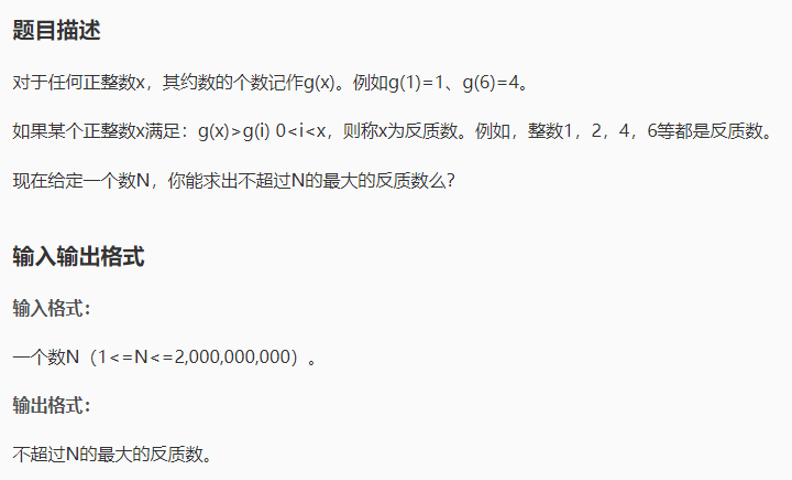
\includegraphics[width=\textwidth, height=\textheight]{luoguP1463.png}
\end{frame}

\begin{frame}{例题1——分析}
 \pause
\begin{itemize}
\item $n$的范围是$2 \times 10^9$,这辈子都不可能想出数学方法的解法了。让我们用打表的思维解决这道题。 \pause
\item 假设$n$很小,那直接读$n$然后直接做。 \pause
\item 我们要做的是枚举$[1,n]$内所有整数,算出它们的约数个数,看看是否满足条件。 \pause
\item 有一个睿智的优化:开一个变量,维护$[1,i-1]$内整数约数个数最大值,每次维护一下即可。 \pause
\item 求一个数的约数个数,要用到约数个数定理: \pause
\item 若一个数$x$唯一分解后等于$\prod_{i=1}^n p_i^{a_i}$,则$x$的约数个数为$\prod_{i=1}^n (a_i + 1)$。
\end{itemize}
\end{frame}

\begin{frame}{例题1——分析}
 \pause
\begin{itemize}
\item 前面的算法复杂度是$O(n\sqrt{n})$的,只能做到十多万的数据。 \pause
\item 那我们如果把这个程序交上去,妥妥地T掉。 \pause
\item 但是我们可以把所有的答案在本地都打出来,存入常量数组,然后就可以二分出答案来了。 \pause
\item 写一个快速打表的程序十分重要,不然你可能一天都打不出表来。 \pause
\item 这种程序只需要跑3min左右。我本来的暴力程序10min还跑没好。 \pause
\item 输出到文件,用C++的语法格式直接输出,然后粘贴到你交的程序中。 \pause
\item 最后的问题就变成了一个sb二分问题了。甚至你都不用二分。
\end{itemize}
\end{frame}

\begin{frame}{例题2:HDU1061}
给你一个正整数$n$,求$n^n$的个位数。$n \leq 1 \times 10^9$。
\end{frame}

\begin{frame}{例题2——分析}
 \pause
\begin{itemize}
\item 这道题看起来就很不可做。让我们用暴力打表看看有没有规律。 \pause
\item 随便打了前1000的答案,然后就发现了规律: \pause
\item 除了第一个数是1,剩下的答案都是有循环节的。 \pause
\item 仔细观察下,一种循环节是901后开始,直到第二个901结束,长度20。 \pause
\item 最后就$n$的大小分类讨论,输出哪个答案即可。
\end{itemize}
\end{frame}

\begin{frame}{作业}
 \pause
\begin{itemize}
\item luoguP1820 寻找AP数
\item luoguP3951 小凯的疑惑
\item luoguP4942 小凯的数字
\item 看luogu日报第59期:我有独特的骗分技巧
\end{itemize}
\end{frame}
\section{随机} % 随机

\begin{frame}{随机}
 \pause
\begin{itemize}
\item 随机算法是一种神奇的算法,也是十分玄学的算法。 \pause
\item 当你需要取出其中的元素进行检验,但又不能规定死了取,这时候我们随机抽取即可。 \pause
\item 这里只介绍低级随机算法。像模拟退火等随机算法就不介绍了。  \pause
\item 随机部分的知识一般不会直接列入考点,但是如何用随机数是很重要的。 \pause
\item 随机的一个重要运用:大名鼎鼎的数据生成器。
\end{itemize}
\end{frame}

\begin{frame}{随机的实现}
 \pause
\begin{itemize}
\item 这里首先要介绍rand函数,这个函数的返回值就是随机数。 \pause
\item 用rand之前要srand。srand需要一个玄学种子作为参数。 \pause
\item rand函数能生成$[0,RAND_MAX]$之间的随机整数,这个$RAND_MAX$多大要看具体的编译器。 \pause
\item 古老的编译器的$RAND_MAX$是32768,现在已经很大了。
\end{itemize}
\end{frame}

\begin{frame}{例题1:luoguP4703}
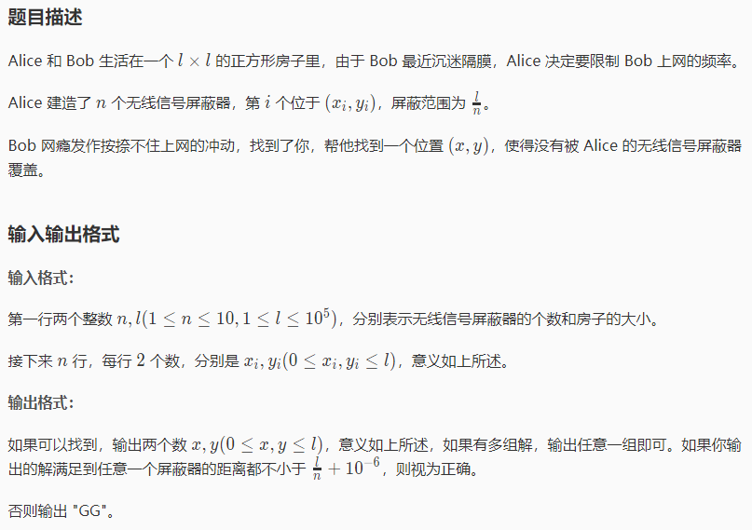
\includegraphics[width=\textwidth, height=\textheight]{luoguP4703.png}
\end{frame}

\begin{frame}{例题2:luoguP2503}
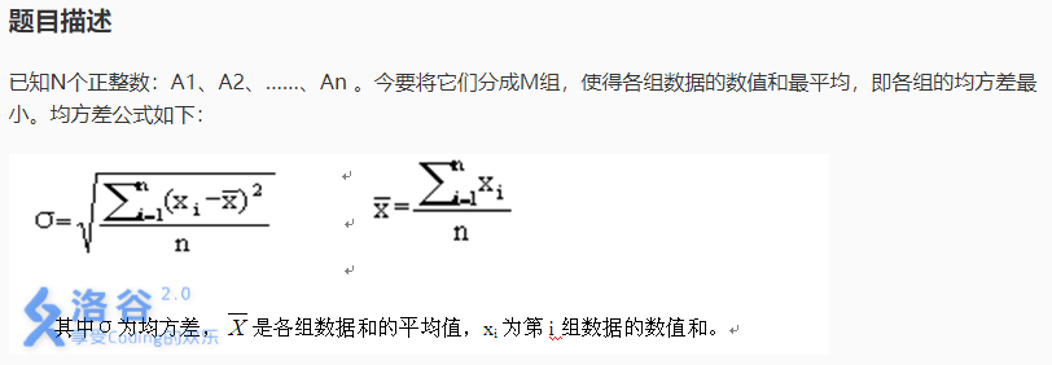
\includegraphics{luoguP2503.png}
\end{frame}

\begin{frame}{例题1、2——分析}
 \pause
\begin{itemize}
\item 第一道题没办法用数组存下来,因为有圆的存在。 \pause
\item 其实随机出里面的点,其实不用随多少次就能搞定。 \pause
\item
\item 第二道题其实只要用一个函数把数据随机打乱,再算均方差即可。 \pause
\item 显然想要答案越正确,你要随更多次,但是要确保不T掉。 \pause
\item 把数据随机打乱有一个STL函数可以做:std::ramdon\_shuffle。 \pause
\item 数据是水的,不用用到模拟退火降温等玄学操作。
\end{itemize}
\end{frame}

\begin{frame}{作业}
 \pause
\begin{itemize}
\item CF1108A Two distinct points
\item 自己学会针对某一道题写数据生成器,数据要保证在数据范围内。
\end{itemize}
\end{frame}
\end{document} 
